\chapter{Краткая заметка на полях по поводу оценок деятельности Александра Македонского}


Значит, смотрите, дело было так. На могучие восточные империи с тысячелетней историей набегают сраные варвары с запада, сносят их одну за другой, разрушают почти каждый крупный город в регионе, уничтожают торговлю, культуру, письменность, и, канешн, людей, причем в товарных количествах. Всё это происходит буквально за полвека, этакое обнуление цивилизации в регионе. И после этого обнуления начинаются первые в истории Темные Века, когда данный плодородный край, одна из колыбелей человечества, приходит в жуткий упадок. Так вот, это я сейчас про Бронзовый Коллапс 1200-1150г до нашей эры. И это то, что НЕ случилось при завоевании эллинами Востока, за что Сашке Македонскому и всем причастным большой респект. 

\begin{figure}[h!tb] 
	\centering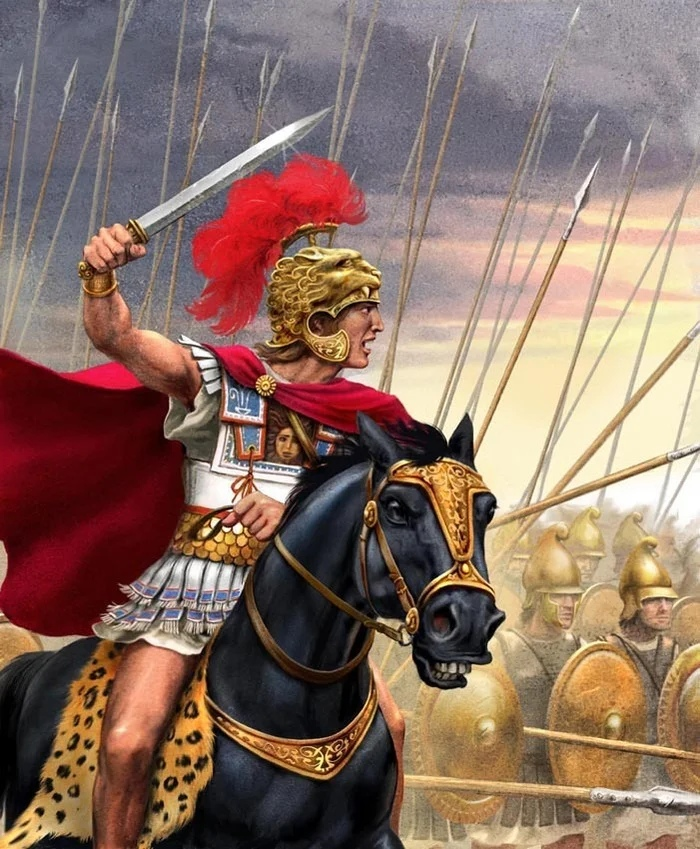
\includegraphics[scale=0.3]{MakedoskiyShort/160153850519581328.png}
	%	\label{fig:scipion} % Unique label used for referencing the figure in-text\end{document}
	%	%\addcontentsline{toc}{figure}{Figure \ref{fig:placeholder}} % Uncomment to add the figure to the table of contents%----------------------------------------------------------------------------------------
	%	\caption{На пикчах ниже всякие вариации на тему "сенаторы убивают Салата".}%	CHAPTER 2
\end{figure}



Македонский, в отличии от своих диковатых предшественников, не пытался Персию снести, разграбить и уничтожить. Он хотел ей править, тоесть кооптироваться в гигантскую и богатую восточную империю, потеснить правящую верхушку и занять её место. Это был, так сказать, "македонский проект", под который он и мобилизовал всю Элладу, и она вписалась в его походы без особого сопротивления (а попытавшиеся бунтовать Фивы он показательно осадил, взял и разрушил), томушта перспективы были реально сказочные. Как говорил Цезарь про восточные походы Помпея: "легко было ему прослыть Великим, воюя с этими людьми, которые не умеют воевать". И воевать персы реально не умели, причем это не вчера началось. Это можно прочитать между строк ещё в "Анабасисе" Ксенофонта, где десять тысяч греков бродят по всей Персии (с населением в десятки миллионов человек), дают всем пизды и флегматично так ищут путь домой. Тоесть небольшая и компактная профессиональная армия, размерами уступающая даже ополчению среднего города, становится для Персии де-факто нерешаемой проблемой. И это за пол века до Македонского. Я думаю, что данное произведение эллинским элитам в определенном смысле открыло глаза и промыло мозги на тему того, что "если десять тысяч наемников там бродят и никто не может им помешать, то почему бы им быть не десятью тысячами, а, скажем, 30-40, и не бродить там, а захватить себе пару сатрапий, например". Ну и после этого началось, собственно. В Элладе при Филиппе, по сути дела, срач был за то, кто возглавит восточный поход, а то что поход будет – это дело решенное.


И вот тут, возможно, рокировка Филиппа на Александра сыграла очень важную роль, так как Филипп - человек старой закалки, в целом рассматривающий Персию как место для "устроить дестрой" пока момент подходящий, пограбить и покарать старого противника. И под его руководством поход, скорее всего, был бы не менее успешен в военном плане (персы реально мало что могли противопоставить грекам на поле боя), но вот последствия могли быть сильно другими, примерно как у Бронзового Коллапса, где Персию бы просто выпотрошили. А вот Александр Филиппыч, родившийся и выросший с мыслью, что "скоро пойдем брать Восток", он как раз продавливал захват Персидской имперки, и воспринимал её не как врага, а как приз. И мысль о том, чтоб там всё сжечь, собрать лут и уплыть обратно в Македонию, коровам хвосты крутить - просто не приходила в голову. Македония эт стартовая точка, а финал истории - это захват и подчинение всего Персидского Мира. И он с этим успешно справился - за пару лет просто снес верхушку и раздолбал лично Дария, после чего объявил себя новым "царем царей". И послал вниз, сатрапиям, простой сигнал о том, что "всё будет как раньше, только теперь мы тут власть, и если будете сидеть спокойно, то всё будет хорошо, а если не будете - то мы вас убьем". На чем, собственно, подчинение Персии и закончилось: эллины интегрировались в восточную сверхимперию, заняли своё место, а потом, после смерти Александра, порвали её на лоскуты и провели первичный передел собственности, запилив вполне жизнеспособные восточные царства.


Такие дела. И вполне возможно, что персы, интуитивно или сознательно, такой исход предсказывали, и именно поэтому старались окультуривать окружающих их варваров по мере возможности. Чтобы в случае подобных эксцессов это было как у Сашки Македонского а не как у "народов моря".

\begin{figure}[h!tb] 
	\centering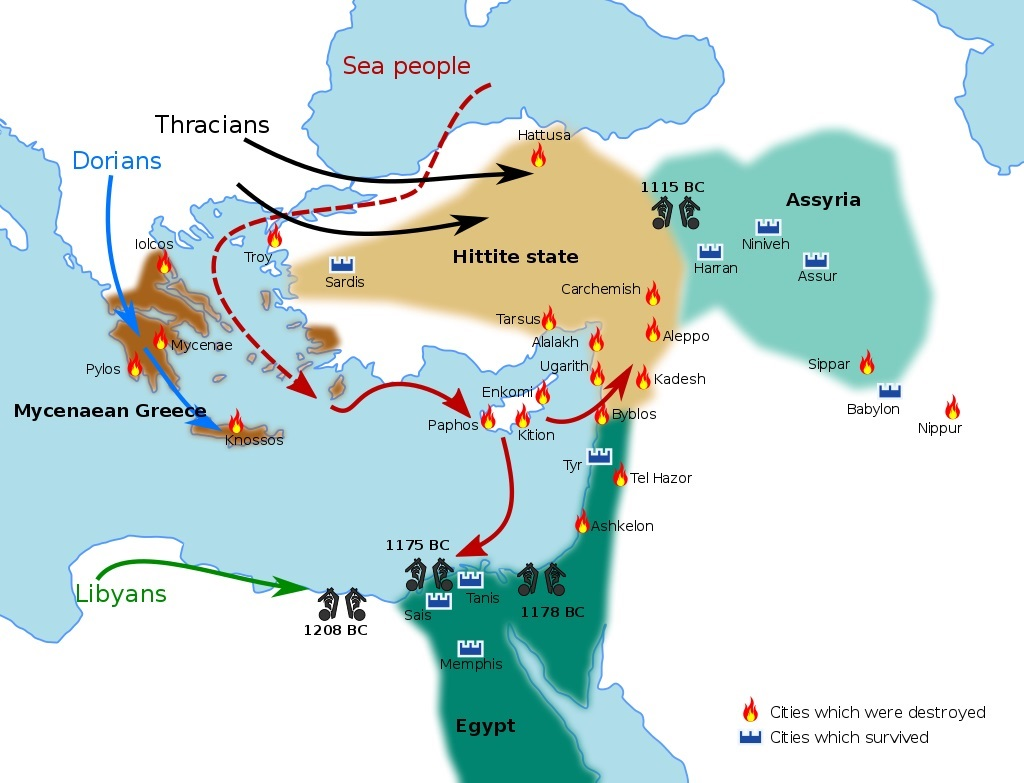
\includegraphics[scale=0.3]{MakedoskiyShort/1601538507153295553.png}
	%	\label{fig:scipion} % Unique label used for referencing the figure in-text\end{document}
	%	%\addcontentsline{toc}{figure}{Figure \ref{fig:placeholder}} % Uncomment to add the figure to the table of contents%----------------------------------------------------------------------------------------
	%	\caption{На пикчах ниже всякие вариации на тему "сенаторы убивают Салата".}%	CHAPTER 2
\end{figure}




Чем-то подобным занимались и имперские римляне на границах по Рейну и Дунаю, о чем я писал уже:[!!!!!!!!!!!!!!!!!!] Религиозный римский гамбит. Это единый сюжет про две дряхлеющие империи, держащие границу от варваров, но понимающие, что однажды она рухнет и эти варвары придут брать своё. Тут самоочевидна схема с "культурной победой", смысл которой в том, чтобы переварить мозги варварам ДО того, как они проломят заслоны и начнут забирать у дряхлеющей державы её регионы. Так как именно от состояния варварских мозгов и будет зависеть результат. "Дикие" варвары просто выжгут всё нахер и скатят захваченное на свой уровень - в Темные Века. А вот "окультуренные варвары" - нет. Они захотят перехватить управление и пользовать захваченное в собственных интересах, а это уже победа.


Разбив Дария, Александр начал входить в "права наследования", а там одно убранство дворцов потянет на десятки годовых бюджетов всей Эллады вместе взятой. Персия всё-таки могучая и древняя цивилизация в богатейшем регионе планеты, а эллины - это просто чутка окультуренные потомки тех самых "народов моря", снесшие в своё время Микенскую цивилизацию и заселившие Греческий архипелаг. После этого эллины своими колониями за несколько веков засрали всё Средиземноморье не от хорошей жизни, а потому что на Малой Греции жить было вообще не сахар. А тут, значит, им падает в руки такой приз, вся Персидская империя. Ну как тут можно всё сжечь, собрать награбленное в мешок и уплыть обратно на свои холодные острова? Да никак, собственно.

\begin{figure}[h!tb] 
	\centering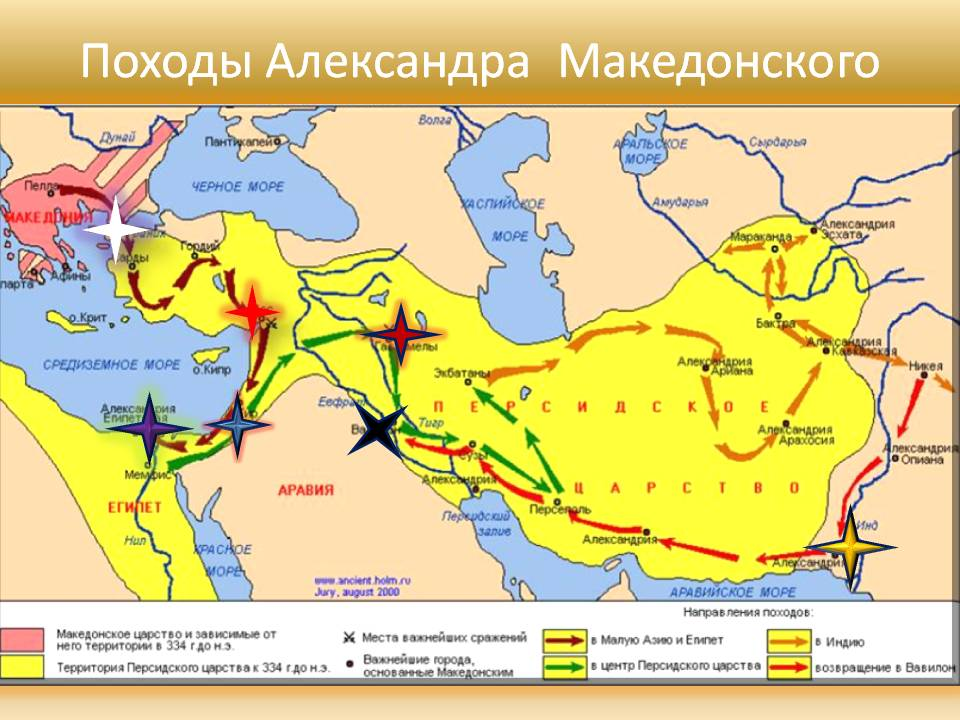
\includegraphics[scale=0.3]{MakedoskiyShort/160153850911471969.png}
	%	\label{fig:scipion} % Unique label used for referencing the figure in-text\end{document}
	%	%\addcontentsline{toc}{figure}{Figure \ref{fig:placeholder}} % Uncomment to add the figure to the table of contents%----------------------------------------------------------------------------------------
	%	\caption{На пикчах ниже всякие вариации на тему "сенаторы убивают Салата".}%	CHAPTER 2
\end{figure}




P. S.

И ещё одно небольшое дополнение. Граждане что моих римлян, что персов недооценивают, видя только один уровень планирования. Мол, "окультурим варваров чтобы когда они нас завоюют - больно не били". И на этом основании обвиняют их в слабоумии. А это только долгосрочные последствия. Хотя и они неплохи, и, де-факто, делают твою цивилизацию условно бессмертной.


На пару этажей пониже у нас другие причины, не столь долгосрочные:


1. Когда ты травишь варваров ядом цивилизации, они менее охотно снимаются со своих стоянок и лезут на тебя дикими толпами, так как начинают нормально обрабатывать земельку и вообще вести оседлый образ жизни.


2. Их общая свирепость тоже снижается, они становятся более договороспособны. Всё ещё не могут в регулярную армию, тоесть тебе ещё не соперник, но уже не могут в "ололо, набег", тоесть уже не столь опасны. Причем этот процесс на столетия, когда рядом с тобой всё ещё грозное, но уже не взрывоопасное варварское королевство, вместо орды.


3. Регулярной армии просто удобно воевать с противником, который имеет постоянные поселения, логистику и экономику, а с живущими в лесу и молящимися колесу германцами - неудобно. Германцев приходится вырезать, там все люди это воины, включая детей. Более культурных варваров можно разбивать в сражениях, убивать их вождей, захватывать их города и принуждать к миру.


4. Следствие предыдущего: территории с цивилизацией банально можно захватить, а их население поработать или прост подчинить. Территории с молящимися колесам дикарями можно только колонизировать, убивая всё живое. Тоесть тут яд цивилизации прокладывает дорогу для военной экспансии.


5. Экономика. Пока территория с варварами не захвачена, с ней можно и нужно торговать, так и гешефт прет и культурка вслед за денюжкой просачивается.


6. Ну и ваши ручные варвары, которых вы приручили одной рукой давая им сахарок вашей культуры и экономического могущества, а другой хуяря их своими легионами по башке, - они замиряются и живут у вас на границе. Держа эту самую границу он других варваров, совсем уж диких и ебанутых. И ценя своё место "на подсосе" у могучей империи, они будут резко против вторжения конкурентов и оттеснения от кормушки.


И только потом, да, вы получаете ещё и точку сохранения на случай смерти. Если ваша граница рухнет, то ваши диковатые соседи не попрут живой волной уничтожать всё на своем пути, а аккуратно и деликатно вступят в права наследования и просто заберут у вас ваши регионы, отправив вас самих на пенсию. Что архиважно, но все таки очень долгосрочно, и я сомневаюсь, что в моменте кто-то этим руководствовался. Но краткосрочные и среднесрочные плюсы окультуривания соседских дикарей - очень вкусные, а значит игра вполне стоила свеч.


В общем, предки были не дурачки, прекратите их таковыми считать.

\begin{figure}[h!tb] 
	\centering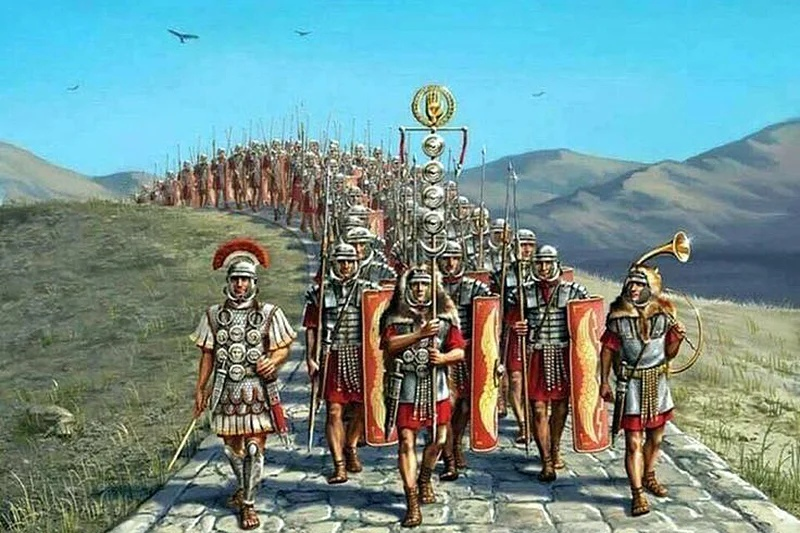
\includegraphics[scale=0.3]{MakedoskiyShort/1601539180132287292.png}
	%	\label{fig:scipion} % Unique label used for referencing the figure in-text\end{document}
	%	%\addcontentsline{toc}{figure}{Figure \ref{fig:placeholder}} % Uncomment to add the figure to the table of contents%----------------------------------------------------------------------------------------
	%	\caption{На пикчах ниже всякие вариации на тему "сенаторы убивают Салата".}%	CHAPTER 2
\end{figure}
